\documentclass[12pt,a4paper,italian]{article}

\usepackage{wrapfig}
\usepackage[italian]{babel} 
\usepackage[T1]{fontenc} 
\usepackage[utf8]{inputenc} % Consente l'uso caratteri accentati italiani
\usepackage{graphicx}
%\usepackage{subfigure}
\usepackage{float}
\usepackage{tabularx,ragged2e,booktabs}
\usepackage{hyperref}
\usepackage{multirow}
\usepackage{notoccite}
\usepackage{tabularx}
\usepackage{subcaption}
\usepackage{amsmath}
\usepackage[outdir=./img/]{epstopdf}
\usepackage{algpseudocode}
\usepackage{algorithm}
\usepackage{amsthm}
\usepackage{amsfonts}
\usepackage{fancyhdr}
\usepackage{appendix}



%--------------------------------------------------------------
%definizione formattazione xml 
%--------------------------------------------------------------
\usepackage{listings}

\usepackage{color}
\definecolor{magenta}{RGB}{220,0,125}
\definecolor{darkblue}{RGB}{60,31,248}
\definecolor{orange1}{RGB}{201,89,0}
\definecolor{lightgray}{RGB}{200,200,200}
\definecolor{gray}{RGB}{125,125,125}

\lstset{
  basicstyle=\ttfamily,
  columns=fullflexible,
  backgroundcolor = \color{lightgray},
  showstringspaces=false,
  commentstyle=\color{gray}\upshape
}

\lstdefinelanguage{XML}
{
  basicstyle=\tiny,
  morestring=[s]{"}{"},
  morecomment=[s]{?}{?},
  morecomment=[s]{!--}{--},
  commentstyle=\color{gray},
  moredelim=[s][\color{black}]{>}{<},
  moredelim=[s][\color{orange1}]{\ }{=},
  stringstyle=\color{darkblue},
  identifierstyle=\color{magenta}
}

%----------------------------------------------------------------


\frenchspacing % forza LaTeX ad una spaziatura uniforme, invece di lasciare più spazio
% alla fine dei punti fermi come da convenzione inglese
\title{\Huge Simulatore dati per Km4City} % \LaTeX è una macro che compone il logo "LaTeX"
% I commenti (introdotti da %) vengono ignorati
\setlength{\parindent}{0pt}
\author{Filippo Ermini\\
	{\tt\small filippo.ermini@gmail.com}\\\small{Università degli Studi di Firenze Scuola di Ingegneria Informatica}\\\\Elaborato per il corso di\\ \emph{Knowledge Management and Protection Systems}\\ Prof. Paolo Nesi\\
	\newline
	\small{Tutor e supervisore Prof. Pierfrancesco Bellini}\\}
\date{Aprile 2017}
%in alternativa a \date il comando \today introduce la data di sistema.

\pagestyle{fancy}
\fancyhf{}
\lhead{\leftmark}
\rfoot{Pagina \thepage}


\fancypagestyle{plain}{%
	\fancyhf{}
	\rfoot{Pagina \thepage}
	\renewcommand{\headrulewidth}{0pt}}



\begin{document}

	\maketitle % Produce il titolo a partire dai comandi \title, \author e \dat
	\thispagestyle{empty}
	
\begin{abstract}
	\begin{center}
		Sviluppo di un componente applicativo, per la generazione di dati simulati per la piattaforma KM4City
	\end{center}
	
\end{abstract}
	\newpage
	\tableofcontents
	\thispagestyle{empty}
	\newpage
	
\section{Introduzione}
\thispagestyle{plain}
L'elaborato riguarda lo sviluppo di un componente applicativo, realizzato in Java, per la piattaforma KM4City funzionale alla generazione di triple rappresentanti una campionatura ad un certo istante di un sensore la cui struttura sia già definita all'interno di KM4City ma del quale non abbiamo ancora a completa disposizione i dati.\\
KM4City è basata su un'ontologia RDF all'interno della quale sono stati definiti i sensori e la loro relativa struttura organizzata in classi e proprietà.\\
Il componente realizzato è in grado di generare un set specifico di dati a partire da un semplice file di configurazione, il quale definisce, attraverso un metalinguaggio specifico dell'applicazione, la tipologia di dato d'uscita e la relativa funzione di generazione.\\
Tramite il file di configurazione andiamo dunque a definire, sulla base della struttura che il sensore ha all'interno dell'ontologia, il valore delle triple \emph{<soggetto,predicato,oggetto>} che andranno
a simulare il campionamento del sensore ad un certo istante.\\
\newline
\newpage
\section{Le Triple RDF}
Gli applicativi di KM4City utilizzano come fonte di dati file di tipo \emph{.n3}, ubicati all'interno di una specifica alberatura di cartelle, 
contenenti la rilevazione ad un certo istante di tempo di un intero set di sensori (tutti appartenenti alla solita classe).

\begin{figure}[!h]
	\centering
	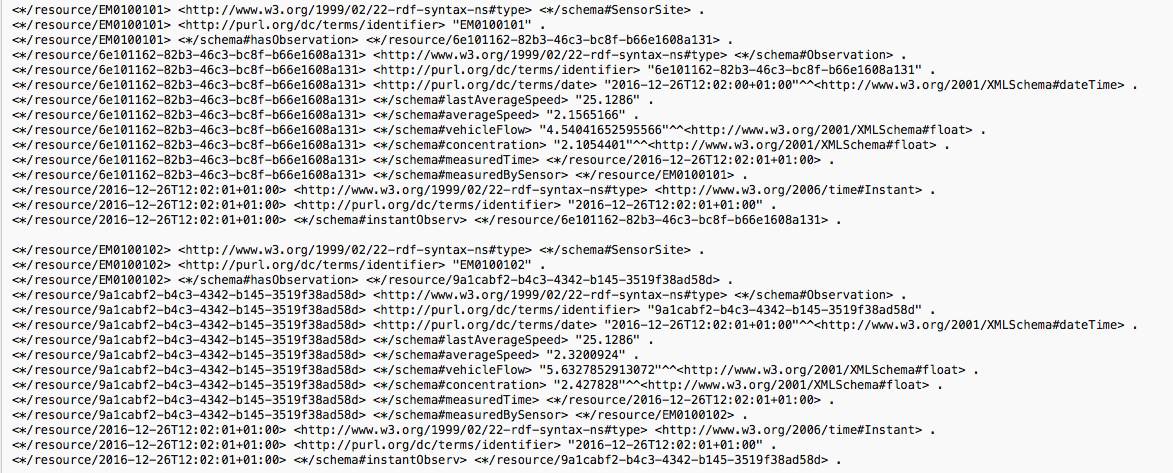
\includegraphics[height=5.5cm]{img/triplerdf2.png}
\caption{\emph{Esempio di un set di triple RDF (per motivi di rappresentazione grafica la stringa} \texttt{http://www.disit.org/km4city} \emph{è stata sostituita con *})}
\end{figure}

Nell'immagine d'esempio sono mostrate due simulazioni relative a due sensori distinti appartenenti alla solita classe (classe dei sensori del traffico). 
Ogni processo di simulazione genera un blocco di triple per ciascun sensore appartenente ad un set predefinito
risultato di un'interrogazione nella base dati RDF.
\subsection{Struttura delle Triple}
Ogni blocco di triple appartenente ad una stessa classe , come vedremo, ha la medesima struttura. Di conseguenza è stato possibile implementare un algoritmo in grado di valorizzare
i tre parametri della tripla che lo compongono (\emph{soggetto, predicato, oggetto}) in modo automatico a partire da alcuni parametri iniziali.\\
Il blocco di triple che descrivono il sensore è composto da: classi (o istanze), attributi della classe e riferimenti ad altre classi.\\
Nell'esempio di figura \ref{triplerdf} è riportato un blocco di triple suddiviso per classi. Ogni classe possiede obbligatoriamente l'attributo\\ \texttt{http://www.w3.org/1999/02/22-rdf-syntax-ns\#type} che identifica la classe alla quale appartiene quella risorsa.
Un altro attributo obbligatorio è \texttt{http://purl.org/dc/terms/identifier}. Il valore di questo attributo identifica l'id della risorsa della classe in questione.
Le altre triple della classe, infine, rappresentano proprietà della classe oppure sono riferimenti a risorse di altre classi.\\
\begin{figure}[!h]
	\begin{subfigure}{1\textwidth}
		\centering
		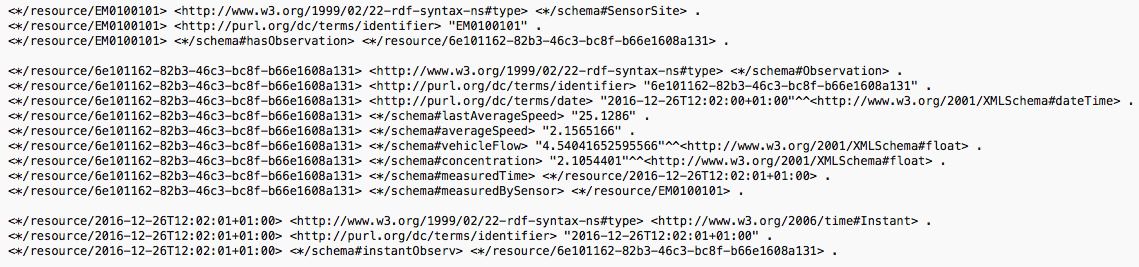
\includegraphics[width=14cm]{img/triple.png}
		\caption{Esempio di triple suddivise per classi RDF}\label{triplerdf}
	\end{subfigure}
	\begin{subfigure}{1\textwidth}
		\centering
		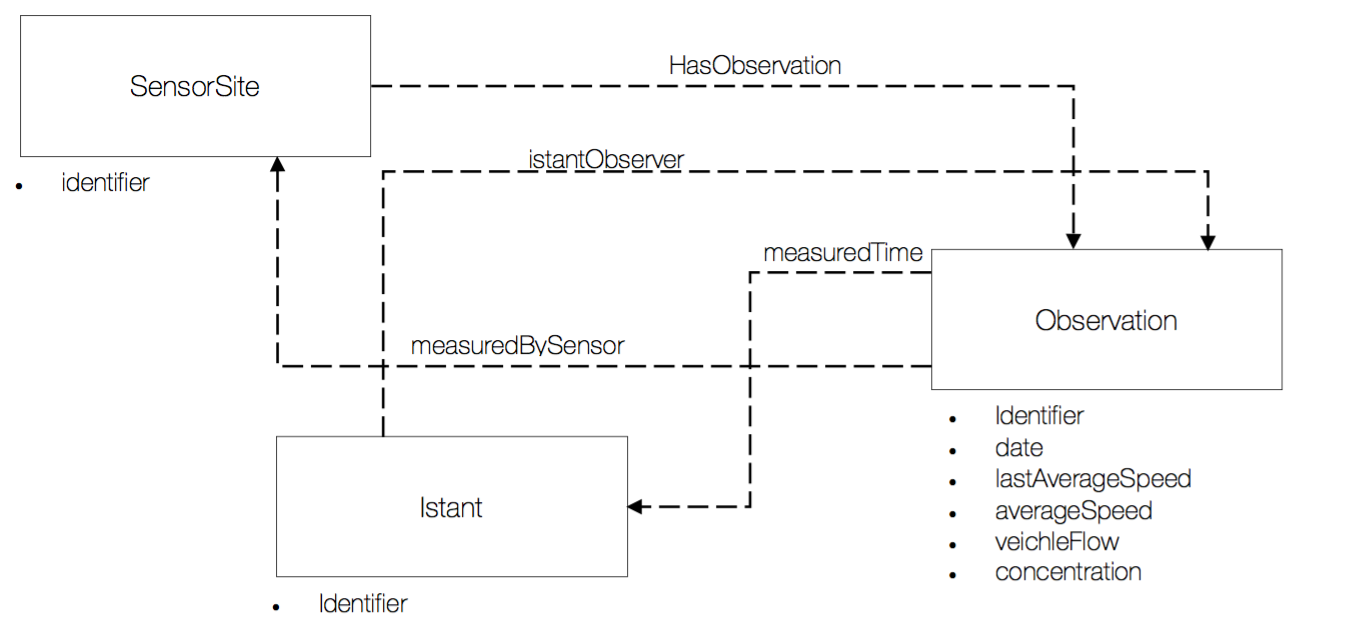
\includegraphics[width=14cm]{img/schema.png}
		\caption{Schema delle classi RDF riferite alle triple dell'esempio precedente}\label{schema}
	\end{subfigure}
	\caption{Triple e schema delle classi RDF}\label{rdfcombo}
\end{figure}
\newline
Nelle due immagini è mostrata la struttura di un esempio di triple RDF utilizzate per descrivere l'informazione relativa ad un sensore di traffico. Il tutto è composto da 3 classi ciascuna delle quali è identificata come una risorsa tramite un identificativo. Per ogni risorsa della classe, sono poi, specificati tutti i suoi attributi, mentre i riferimenti verso le altre classi (le frecce tratteggiate nello schema \ref{schema}) contengono come valore l'\emph{identifier} della risorsa alla quale fanno riferimento. 
\newpage

\section{Il File di Configurazione}
A fronte di quanto detto nel paragrafo precedente è stato implementato un algoritmo in grado di generare, in modo sistematico, una simulazione della campionatura in ordine ad un qualsiasi  sensore già definito all'interno dell'ontologia a partire da un file nel quale un utente esperto, cioè un utente che ha un'ampia conoscenza dell'ontologia di \emph{KM4City}, specifica come devono essere valorizzate le proprietà 
delle classi che definiscono il sensore. Tale file è scritto con la sintassi \emph{XML}.

\subsection{Struttura del file XML}
A seguito è descritta la struttura gerarchica dei nodi e delle loro proprietà che compongono il file di configurazione.\\

\begin{figure}[h!]
	\centering
	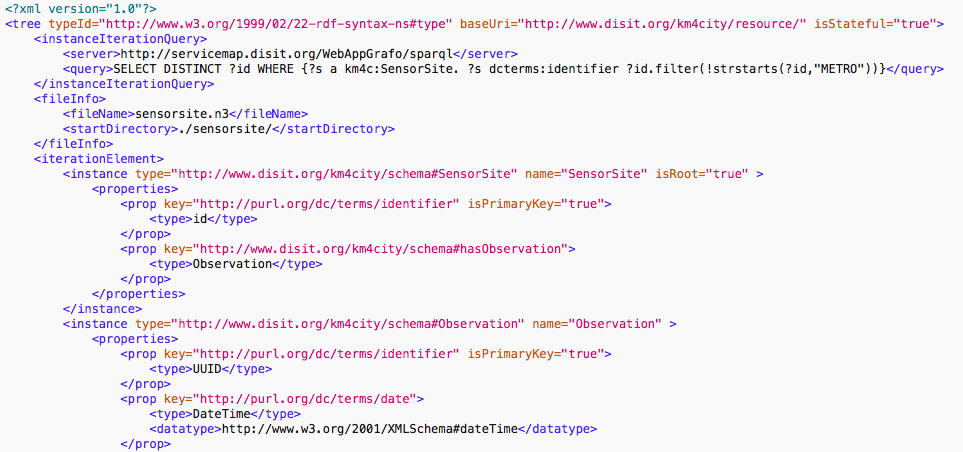
\includegraphics[width=14cm]{img/configxml.png}
	\caption{Estratto di un file di configurazione xml}\label{configxml}
\end{figure}

\subsubsection{<tree>}
\`E l'elemento radice ed ha le seguenti proprietà:
\begin{itemize}
	\item \textbf{typeId}: [Obbligatorio] Il suo valore indica l'\texttt{URI} da usare per indicare la tipologia della classe, ovvero, in altre, parole il valore del complemento della tripla 
	che deve indicare il tipo della classe.
	\item \textbf{isStateful} [Opzionale] Se true crea un file \emph{json} con tutti i valori dell'ultima esecuzione, tale file può essere riutilizzato in esecuzioni successive per tenere conto dei valori 
	precedentemente generati (le specifiche di questa funzionalità sono descritte a seguire nel paragrafo relativo alla tipologia \textbf{previusstate}). 
\end{itemize}
\subsubsection{<fileInfo>}\label{fileinfo}
Questo elemento definisce le specifiche del file di uscita, e deve contenere i seguenti elementi:
\begin{itemize}
	\item \textbf{FileName} [Obbligatorio] Specifica il nome del file \emph{.n3} d'uscita.
	\item \textbf{StartDirectory} [Obbligatorio] \`E la cartella all'interno della quale verranno generati i file risultato della simulazione.
\end{itemize}
A partire dalla cartella specificata sarà creata un'alberatura di cartelle con il seguente formato: \texttt{AAAA\_MM\textbackslash GG\textbackslash HH\textbackslash mmss\textbackslash filename.n3}, dove i simboli rappresentano i valori di data e e ora.


\subsubsection{<instanceIterationQuery>}
Questo elemento contiene  la definizione di una query SPARQL. Al suo interno si specifica la query SPARQ, i cui risultati rappresentano la lista di sensori sui quali iterare.
La query deve avere una struttura tale da restituire in uscita una lista di identificativi che rappresentano i sensori per i quali si vogliono generare delle simulazioni.\\
Questo elemento non possiede proprietà ma deve aver valorizzati i seguenti elementi:
\begin{itemize}
	\item \textbf{query} [Obbligatorio] Query sparql
	\item \textbf{server} [Obbligatorio] End-point a cui sottoporre la query
	\item \textbf{bindingValue} [Opzionale] Campo della select su cui andare a recuperare il valore d'uscita (default = id)
\end{itemize}

\subsubsection{<iterationElement>}\label{itarationelement}
\`E l'elemento che contiene le definizioni della struttura RDF e le regole di generazione dei valori del sensore. Per ogni elemento generato dalla query si
rieffettua una generazione dei dati secondo le regole definite all'interno di questo elemento.\\
All'interno di questo elemento si definiscono quindi le istanze e le proprietà del sensore in accordo con la struttura della base dati RDF.\\
Questo oggetto contiene 2 tipologie di elementi:
\begin{itemize}
	\item \textbf{attributes} [Opzionale] Questo elemento contiene una lista di proprietà che non si riferiscono direttamente alla struttura RDF ma sono degli attributi 
	di supporto alla generazione dei valori delle proprietà del sensore. Talvolta può accadere che il valore di alcuni attributi sia il risultato di una combinazione di fattori la cui generazione 
	risulterebbe complicata se eseguita in una sola volta. L'idea che sta alla base dell'utilizzo di questa funzionalità è di poter demandare la generazione di quei valori, il cui risultato è funzione di più elementi,
	in questa sezione per poi referenziarli nella proprietà opportuna.\\
	Un caso emblematico in cui è utile dichiarare una variabile di appoggio in questa sezione, è quello in cui un valore sia funzione del risultato di una query e che in aggiunta debba subire elaborazioni successive. Per casi come questi, a meno che non sia possibile eseguire l'elaborazione del dato direttamente dalla query \texttt{SPARQL}, si può dichiarare in questa sezione una variabile che conterrà il risultato della query e nell'apposita proprietà (all'interno dell'istanza di cui fa parte) il valore verrà determinato attraverso una espressione, funzione della variabile che abbiamo dichiarato in questa sezione.
	\item \textbf{list<istance>} [Obbligatorio] Lista delle istanze che definiscono la struttura del sensore. In questa sezione si definiscono le istanze (rappresentanti le classi) e 
	le proprietà ad esse associate necessarie a definire l'intero oggetto (sensore) RDF. Le istanze contengono le informazioni necessarie a definire la tripla. Ognuna di esse contiene 
	una lista di proprietà dove per ognuna di esse sono definite oltre alle informazioni utili a generare la tripla anche le regole di generazione del valore del singolo attributo.
\end{itemize} 
\subsubsection{<istance>}
Elemento che definisce la struttura e gli attributi di un'istanza RDF.\\
Proprietà:
\begin{itemize}
	\item \texttt{type}: valore dell'uri \emph{rdf-syntax-ns\#type} dell'istanza.
	\item \texttt{name}: nome attribuito all'istanza utilizzato per richiamarla all'interno di altre istanze. 
	\item \texttt{isRoot}:se true indica se questa istanza contiene l'elemento su cui inserire il valore generato dalla query.
	\item \texttt{baseUri}: valore del \emph{baseURI} dell'istanza.
\end{itemize}
Elementi:
\begin{itemize}
	\item \textbf{properties} [Obbligatorio] Elemento che contiene la lista di attributi che definiscono l'istanza.
\end{itemize}
\subsubsection{<properties>}
Contiene la lista delle proprietà dell'istanza.
\begin{itemize}
	\item \textbf{list<prop>} [Obbligatorio]
\end{itemize}

\subsubsection{<prop>}
Con questo elemento si specificano le singole proprietà dell'istanza e come esse devono essere generate. Per ognuna di esse sono stati definiti dei campi utili alla generazione dei valori della tripla RDF ed altri campi necessari alla generazione del valore dell'attributo. Come vedremo in seguito sono stati individuati alcuni tipi con cui una proprietà può essere
definita. Ogni tipo necessita di ulteriori attributi definiti ad hoc per quella tipologia, utili alla generazione del valore di uscita.\\
Proprietà:
\begin{itemize}
\item \texttt{key}: valore della uri del predicato di quell'attributo.
\item \texttt{isPrimary}: se \emph{true} indica che quell'attributo è chiave primaria per l'istanza a cui appartiene (solo un attibuto per istanza può essere chiave primaria).
\end{itemize}
Elementi:
\begin{itemize}
\item \textbf{type} [Obbligatorio]: indica il tipo di valore che deve essere generato (ogni tipo può necessitare elementi aggiuntivi).
\item \textbf{uri} [Obbligatorio]: valore dell'oggetto della tripla RDF.
\item \textbf{format} : valore contenente la stringa con sintassi ''C-like'' del formato di uscita (e.g. ''\%.3f''). Il valore generato verrà dunque formattato in funzione della stringa definita all'interno dell'elemento.
\end{itemize}

\subsection{Lista Tipi}
La generazione dei valori può avvenire in molti modi: per cercare di offrire la maggiore capacità espressiva sono state implementate molteplici tipologie 
per la generazione pseudo-casuale dei valori delle proprietà.
Ognuno dei tipi sotto elencati può essere utilizzato come tipo di valore d'uscita per quella specifica proprietà.Sarà sufficiente specificarlo 
nell'attributo \emph{type} con a seguito i parametri di cui necessita.\\

\subsubsection{id}  Definisce che la proprietà dovrà contenere il valore proveniente dalla query di iterazione, 
questa proprietà deve essere attribuita all'istanza con \emph{isRoot = true}.\\
Parametri aggiuntivi: Nessuno
\subsubsection{integer} L'attributo restituirà un valore intero generato casualmente in un intervallo.\\
Parametri aggiuntivi:
\begin{itemize}
	\item \texttt{maxValue}: Estremo superiore dell'intervallo.
	\item \texttt{minValue}: Estremo inferiore dell'intervallo.
\end{itemize}
\subsubsection{float} L'attributo restituirà un valore float generato casualmente in un intervallo.\\
Parametri aggiuntivi:
\begin{itemize}
	\item \texttt{maxValue}: Estremo superiore dell'intervallo.
	\item \texttt{minValue}: Estremo inferiore dell'intervallo.
\end{itemize}
\subsubsection{md5} Genera il valore md5 di una stringa\\
Parametri aggiuntivi:
\begin{itemize}
	\item \texttt{md5String}: Contiene la stringa da crittografare
\end{itemize}
\subsubsection{datetime} 
Tipologia che genera una data in formato ISO 8601, se non specificati gli estremi dell'intervallo la data assume il valore dell'istante in cui è generata, altrimenti genera un valore casuale nell'intervallo di date.
Parametri aggiuntivi:
\begin{itemize}
	\item \texttt{maxValue}: Estremo superiore dell'intervallo.
	\item \texttt{minValue}: Estremo inferiore dell'intervallo.
\end{itemize}
\subsubsection{hourdependent} Questa tipologia serve a generare dei valori diversi per ogni ora della giornata in base a dei valori orari di riferimento specificati.
Parametri aggiuntivi:
\begin{itemize}
	\item \texttt{hourValue}: Contiene i valori di riferimento per ogni ora. Devono essere inseriti 24 valori separati da ';'. 
	\item \texttt{range}: Contiene il range di variazione all'interno del quale possiamo far variare il valore di riferimento indicato. Può essere un
	valore unico per tutti e 24 i valori oppure può essere definito in modo analogo a hourValue indicando i 24 valori del range.
\end{itemize}
\subsubsection{profiledependent} \label{profiledependent}Con questa tipologia, che è concettualmente molto simile alla precedente, è possibile generare il valore di un attributo a partire da un set di profili normalizzati (tra 0 - 1) definiti per specifici giorni della settimana con
valori campionati ad intervalli di 15 minuti (96 campionature) che dovranno essere infine moltiplicati per un valore di riferimento. Questi valori sono specificati in file in formato \emph{.csv} che deve essere importato dal sistema.\\
\begin{figure}[!h]
	
	\begin{subfigure}{.3\textwidth}
		\centering
		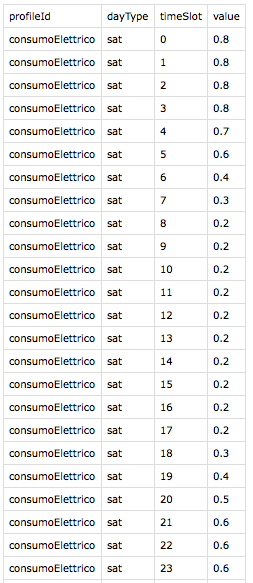
\includegraphics[width=.8\linewidth]{img/profilo1.png}
	\end{subfigure}
	\begin{subfigure}{.3\textwidth}
		\centering
		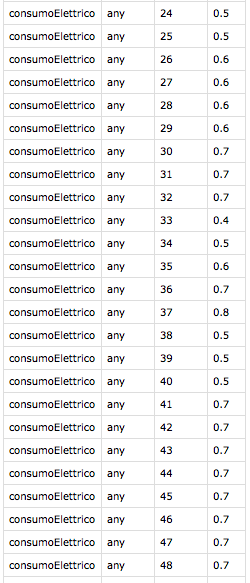
\includegraphics[width=.8\linewidth]{img/profilo3.png}
	\end{subfigure}
	\begin{subfigure}{.3\textwidth}
		\centering
		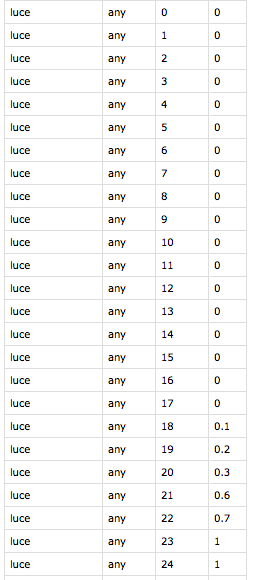
\includegraphics[width=.8\linewidth]{img/profilo2.png}
	\end{subfigure}
	\caption{Alcuni estratti del contenuto di un file \emph{.csv}}\label{csvfile}
\end{figure}
All'interno di un file \emph{.csv} possono essere definiti più di un profilo (e.g. ''consumo elettrico'', ''luce'', ''umidità''  ecc...) per ognuno di questi sono definiti i valori giornalieri di riferimento. La distinzione dei giorni può essere fatta specificando dei profili diversi per i diversi giorni della settimana oppure specificando un profilo \emph{any} valido per tutti i giorni per i quali non è definito un profilo. Come nel caso precedente anche qui dobbiamo definire un valore che specifica l'entità del rumore da aggiungere al valore di riferimento. Il valore finale è ottenuto quindi moltiplicando il valore ottenuto dal profilo in base all'orario per un valore di riferimento, tutto sommato con una perturbazione randomica di ampiezza specificata.\\
Parametri aggiuntivi:
\begin{itemize}
	\item \texttt{profilesFile} Contiene il nome del file \emph{.csv} da utilizzare
	\item \texttt{profileId} Indica quale è il profilo da considerare
	\item \texttt{maxValue} Valore base di riferimento 
	\item \texttt{variance} Valore della varianza 
\end{itemize}  

% esempio di file csv 

\subsubsection{fromset} 
Con questa tipologia si estrae un valore a caso da un set di elementi (se il set contiene un solo elemento sarà estratto sempre quello).
Parametri aggiuntivi:
\begin{itemize}
	\item \texttt{set} Lista di valori separati da ';'.
\end{itemize}
\subsubsection{query} Il valore dell'attributo è il risultato dell'esecuzione di una query (la query deve restituire un solo valore).\\
\newline
\emph{Elemento della stessa tipologia di \textbf{instanceIterationQuery}, con la sola differenza che in questo caso la query deve restituire un solo record e non una lista.}\\
\subsubsection{valueexpression} Definendo un attributo con questa tipologia si permette di definire il valore di un attributo come risultato di una espressione  algebrica o logica contenete variabili.\\
 Nel caso in cui si necessiti di calcoli più complessi rispetto ad una semplice espressione algebrica è possibile inserire del codice Javascript da far eseguire al sistema.
\\Parametri aggiuntivi:
\begin{itemize}
	\item \texttt{valueExpression} Contiene l'espressione algebrica o logica da eseguire. Le variabili devono essere dichiarate con la seguente sintassi \$\{nome\} dove nome è il valore inserito nelle proprietà dell'attributo prop
\end{itemize}
In caso di espressioni algebriche il valore restituito è sempre di tipo float.\\
Per una descrizione più approfondita delle variabili ed espressioni rgolari si rimanda al capitolo 3.3 .
\subsubsection{foregoing} Attraverso questa tipologia si può andare a referenziare il valore di una variabile generata in passi precedenti all'interno della stessa query di iterazione.\\
Lo scopo di questa tipologia è di permettere di referenziare all'interno di una iterazione un valore generato per un altro sensore sempre all'interno dello stesso ciclo di iterazione corrente.\\
Parametri aggiuntivi:
\begin{itemize}
	\item \texttt{defaultValue}: Valore da usare nel caso in cui l'attributo interessato non sia presente oppure non sia ancora stato generato.
	\item \texttt{refValue}:contiene la coppia \emph{iterazione - nomeVaribile} da cui prendere il valore. Il valore di iterazione può essere sia un intero, che rappresenta l'indice dell'iterazione 
	da cui prendere il valore, oppure l'id del sensore da cui prendere il valore interessato che viene specificato con la variabile nomeVariabile: il tutto con la sintassi \@[iterazione]\{nomeVariabile\}.
\end{itemize}
\subsubsection{previusstate}\label{previusstate} Questa tipologia ha un funzionamento simile alla precedente, con la differenza che in questo caso si può andare a referenziare valori generati in esecuzioni precedenti e non all'interno della stessa esecuzione.
Questa tipologia è utile per generare i valori di quegli attributi che hanno una dipendenza funzionale da stati precedentemente generati. Per fare in modo di poter utilizzare questa tipologia è necessario che sia settato a true la proprietà 
\emph{isStateful} nell'elemento \texttt{<tree>}. Così facendo il programma creerà un dump (in un file esterno in formato json) delle variabili generate ad ogni esecuzione in modo da poter recuperare il valore interessato e poterlo
utilizzare nell'iterazione corrente.
Parametri aggiuntivi:\\
\begin{itemize}
	\item \texttt{defaultValue}: Valore da usare nel caso in cui il valore interessato non sia presente oppure nel caso in cui non esista un'iterazione precedente a quella in oggetto.
	\item \texttt{refValue}:contiene la tripla \emph{indice - idSensore - nomeVaribile} da cui prendere il valore. L'\texttt{indice} specifica quale iterazione precedentemente generata si deve considerare (il conteggio avviene considerando l'iterazione corrente la 0 e la 1 quella precedentemente generata).
Ogni iterazione contiene una lista sensore; quindi è necessario specificare a quale sensore si fa riferimento tramite l'\texttt{idSensore} ed infine è necessario specificare il \texttt{nome} della proprietà che si vuole ottenere.
La sintassi da utilizzare per definire questa query di ricerca è la seguente: \#[indice][idSensore]\{nomeVariabile\}.\\
	\end{itemize}
	
\subsection{Variabili e Espressioni Algebriche}
Talvolta accade che i valori di alcune proprietà abbiano delle dipendenze funzionali da altri valori e che se ne debba tenere conto durante la fase di generazione.
I valori che sono generati per le proprietà delle classi sono valori estratti casualmente: anche se ne viene definito l'intervallo all'interno del quale variare, sono pur sempre valori casuali. 
Per quei valori che sono funzione di altri quindi deve essere introdotta una dipendenza dal valore generato casualmente.\\
Un esempio è il caso dei sensori dei parcheggi, i quali restituiscono informazioni sulle statistiche di utilizzo delle strutture. 

\begin{figure}[h!]
	\centering
	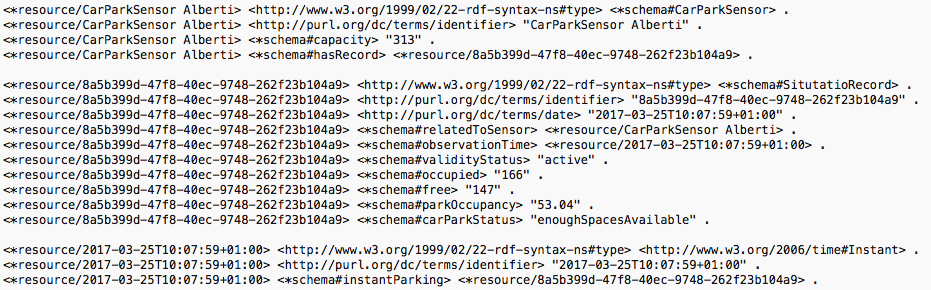
\includegraphics[width=14cm]{img/carParkSensor.png}
	\caption{Esempio di campionatura per un sensore di parcheggio}\label{carparksensor}
\end{figure}

Il valore principale che deve essere generato casualmente è il  ''\emph{numero di posti occupati}'', di conseguenza valori come \emph{numero di posti liberi} e \emph{percentuale di occupazione} devono essere funzione del valore casuale generato in precedenza.\\
Per risolvere questo tipo di problematiche è stata introdotta la possibilità di referenziare valori di proprietà già generati attraverso delle variabili e la possibilità di 
inserire espressioni algebriche.\\
Per ogni proprietà definita è necessario specificare un nome e per referenziare quel valore all'interno di altre proprietà si deve utilizzare la seguente sintassi: \$\{\emph{Nome\_Proprietà}\}
I valori nei quali è inserita una dipendenza funzionale saranno calcolati solo dopo aver generato tutte le loro dipendenze e nei casi in cui è necessario sarà possibile eseguire delle espressioni per determinare il valore di tali proprietà.
\newpage

\section{L'applicativo Java}
Tutto il sistema descritto nei capitoli precedenti è stato realizzato attraverso un applicativo Java. A partire dal file di configurazione questo applicativo genera il file \emph{.n3} per KM4City.\\ In questo capitolo saranno descritti i componenti principali che  compongono l'applicativo.\\
\newline
Il progetto è composto da 3 componenti principali:\\
\begin{enumerate}
	\item \emph{Main}. Classe principale, si occupa di avviare il processo di generazione della simulazione e scrivere i risultati su file.
	\item \emph{Classi per la gestione del dominio dei dati e dei formati}. In questo applicativo si parte da un informazione di base rappresentata in formato \texttt{XML} e inoltre ci sono altri due tipologie di formati che devono essere gestiti: \texttt{JSON e CSV}. Per ognuno dei formati sono state definite delle classi per la relativa gestione. 
	\item \emph{Classi per la gestione delle tipologie}. Sono l'insieme delle classi implementate per poter astrarre dalla conoscenza degli aspetti delle diverse tipologie di dato definite in modo da considerare le singole proprietà delle singole istanze come oggetti generici all'interno del processo iterativo di generazione delle triple.
\end{enumerate}
	\subsection{Main}
	Classe contenente il metodo omonimo che insieme alla classe \texttt{DataSimulator.java} si occupa: dell'acquisizione dei parametri iniziali, di fare partire il processo di generazione dei delle triple e di scrivere il file {.n3}. \\
	
	\texttt{java -jar sensorGenerator.jar -x sensor.xml -n simulazione\_parcheggi} \\
	
	Questa è la stringa con la quale viene lanciato il programma da linea di comando, sono necessari due parametri:\\
	\begin{enumerate}
		\item \texttt{-x} indica il file di configurazione xml (obbligatorio)
		\item \texttt{-n} nome della simulazione (opzionale)
	\end{enumerate}  
	
	La classe \texttt{main} valida gli argomenti passati in ingresso e successivamente istanzia un oggetto della classe \texttt{DataSimulator.java}.
	In quest'ultima si importa il file di configurazione all'interno di un oggetto e si da il via la processo di generazione delle triple, che una volta concluso, -se non si sono verificati errori- genera una stringa con tutte le triple. \\Una volta che questa è stata generata si crea (se non è già stato fatto) le cartelle utilizzando i valori di data e ora (cfr. capitolo \ref{fileinfo}). Infine viene creato il file \texttt{.n3}.\\
	\newline
	Nel caso di esecuzione con memoria (cfr. capitolo \ref{previusstate}) i file \texttt{JSON} delle esecuzioni precedenti vengono importati in un'apposita lista al momento dell'importazione del file di configurazione e il file \texttt{JSON} relativo all'iterazione corrente viene generato al termine dell'esecuzione nella solita cartella che contiene il file \texttt{.n3}.
	
	\subsection{Classi per la gestione del dominio dei dati e dei formati}
	All'interno di questo applicativo sono utilizzati tre tipologie di formati per l'interscambio di dati (\texttt{XML, JSON, CSV}), ognuno di essi utilizzato all'interno di un contesto diverso. Al fine di avere una gestione ottimale delle proprietà dei differenti formati, per ognuno di essi sono state definite delle classi che ne definiscono il comportamento.
	
	\subsubsection{XML}\label{xml}
	Questo formato è il formato utilizzato per definire il file di configurazione. Per gestire questo aspetto è stata definita la classe \texttt{Tree.java}, che contiene  la mappatura dei nodi della struttura del file \texttt{.xml}. Tramite questa mappatura un file \texttt{xml}, se rispetta la struttura definita, verrà serializzato all'interno di un oggetto di tipo \texttt{Tree} (figura \ref{treeClass}).\\
	\begin{figure}[h!]
		\centering
		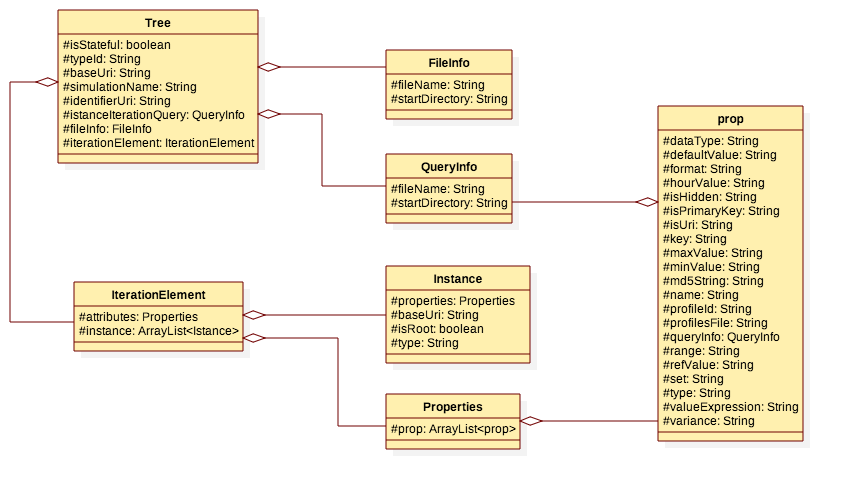
\includegraphics[width=14cm]{img/tree.png}
		\caption{Class Diagram della classe Tree}\label{treeClass}
	\end{figure}
	Per gestire i file di tipo \texttt{XML} è stata utilizzata la libreria esterna JAXB\footnote{Java Architecture for XML Binding (JAXB) - \url{https://jaxb.java.net}} che mette a disposizione le funzioni di serializzazione/deserilizzazione (Marshaller/Unmarshaller nel caso specifico) che sono utilizzate nella classe \texttt{XMLParsing.java} per importare un file in un oggetto di tipo \texttt{Tree}.
	
	\newpage
	\subsubsection{JSON} 
	Questo formato è utilizzato per gestire il caso dell'esecuzioni con memoria; se la proprietà \texttt{isStateful} del nodo \texttt{tree} è settata a \emph{true} si attiva la generazione dei file \texttt{JSON} contenenti il \emph{dump} dell'esecuzione corrente, ognuno di questi file viene salvato insieme al file \texttt{.n3} per poi essere importato all'interno di esecuzioni successive in modo da mettere a disposizione dell'esecuzione corrente anche lo stato assunto da esecuzioni precedenti.\\
	\begin{figure}[h!]
		\centering
		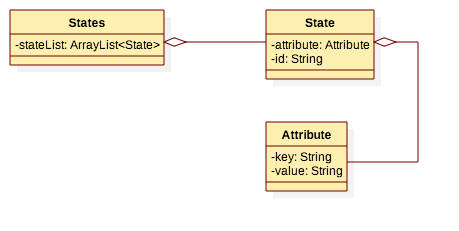
\includegraphics[height=5cm]{img/json.png}
		\caption{Class Diagram della classe per la gestione dei file json}\label{jsonClass}
	\end{figure}\\
	Per gestire i file di questo tipo in Java è stata utilizzata la libreria
	esterna GSON\footnote{Gson is a Java library that can be used to convert Java
		Objects into their JSON representation - \url{https://github.com/google/gson}}.
	Queste classi sono state definite per poter creare un \emph{dump} di una
	esecuzione in un file \emph{json}. I valori relativi ad un singolo sensore sono
	inseriti all'interno di una lista di coppie \emph{<nome\_propriet\'a,valore>} tutto
	all'interno di un oggetto di tipo \texttt{State}. Questo oggetto contiene i
	dati relativi alla campionatura di un sensore, quindi per ogni sensore della
	lista verrà generato un oggetto di tipo \texttt{State}. L'insieme di tutti
	questi oggetti generati è inserito in una lista all'interno dell'oggetto della
	classe \texttt{States}. Questo oggetto è quello che alla fine del processo, in
	caso di esecuzione con memoria, è serializzato in un file \emph{json} tramite
	le API GSON.\\
	In modo duale nel momento in cui si devono importare le storicizzazioni
	precedenti, si esegue una scansione all'interno della cartella, per importare
	in modo ordinato, tutti i file \emph{json} precedemente creati. I file
	importati sono inseriti in una lista di oggetti di tipo \texttt{States}.
	
	\subsubsection{CSV}
	Anche per questa tipologia di formato sono state definite delle classi atte alla gestione di questi file. Un file \emph{csv} è un file contenete dati in formato testo organizzati in colonne. La struttura delle colonne viene realizzata separando gli elementi di una riga attraverso una virgola.\\
	Questa tipologia di file viene utilizzata nel tipo \texttt{profiledependent} (crf. capitolo \ref{profiledependent}), dove nella definizione della proprietà si specifica anche un file \emph{csv} esterno contenete valori di riferimento organizzata in intervalli di 15 minuti raggruppati con profili giornalieri. Un file \emph{csv} può contenere  profili relativi a più contesti (e.g. consumo elettrico, gas, acqua ecc.) e per di differenti giorni della settimana.
		\begin{figure}[h!]
			\centering
			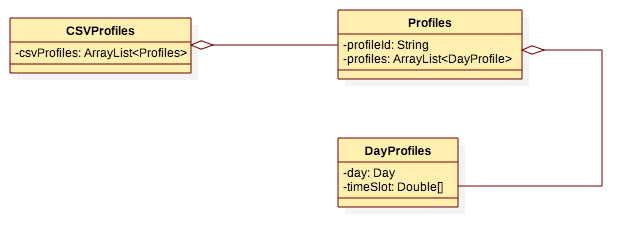
\includegraphics[height=4.5cm]{img/csv.png}
			\caption{Class Diagram della classe per la gestione dei file csv}\label{csvClass}
		\end{figure}\\
	La classe Java che risponde a questa esigenza è la classe \texttt{CSVProfiles}; la quale contiene, in una lista, l'insieme dei diversi contesti presenti all'interno del file \emph{csv}.
	Ogni elemento della lista è un oggetto della classe \texttt{Profiles} la quale contiene tutti i profili giornalieri definiti per un contesto.\\ I profili giornalieri sono organizzati in giorni della settimana ognuno contenente l'array dei \emph{timeSlot} con i 96 valori ( un valore ogni 15 minuti).\\
	La manipolazione di questi dati è unilaterale, i dati sono solo letti non vi è una esportazione come nel caso del \emph{json}. L'importazione del file avviene leggendo il file, non sono utilizzate librerie esterne come nei precedenti casi.
	
	\subsection{Classi per la generazione della simulazione}
	Le classi descritte in questa sezione si occupano della generazione delle triple RDF. A partire da un oggetto di tipo \texttt{Tree}, in base alle specifiche contenute in esso, si genera una campionatura per ogni record restituito dalla query SPARQL.\\
	L'aspetto principale di questo processo è la capacità di poter astrarre dalle specifiche di generazione delle diverse tipologie di dato.\\ Avendo definito un'interfaccia comune per 	ognuna di esse, si demanda la conoscenza dei dettagli specifici della tipologia, alla definizione delle stesse e non al processo iterativo in questione.\\
	Per implementare questo sistema è stato necessario per prima cosa definire delle classi apposite che riprendono la struttura di cui è composta la classe \texttt{Tree}. Questo passaggio si è reso necessario al fine di creare degli oggetti che contenessero,insieme alle proprietà delle istanze e degli attributi, anche i valori generati e dei parametri accessori funzionali alla generazione dei valori stessi.
	
	\subsubsection{IterationElment e IterationManager}
	Queste due classi sono il fulcro principale del processo di generazione delle triple RDF. La classe \texttt{IterationElement} contiene la struttura degli elementi sui quali si deve ciclare, mentre la classe \texttt{IterationManager} si occupa del processo di generazione a partire da un oggetto di tipo \texttt{IterationElement}.
	
	\paragraph{IterationElement}

	In questa classe sono contenute le informazioni sulla struttura degli elementi sui quali si deve iterare, è composta principalmente da due liste: a) la lista di istanze che descrivono l'oggetto; b) la lista degli attributi comuni definiti come supporto alla generazione dei valori principali (crf capitolo \ref{itarationelement}).
	Gli oggetti contenuti all'interno delle due liste alla fine del processo (processo che vedremo nel paragrafo successivo) conterranno anche il valore generato. 
	
	%diagrammclass di iteration element
	
	\paragraph{IterationManager}
	
	Questa classe a partire da un elemento di tipo \texttt{IterationElement} si occupa di generare tutti i valori per tutte le proprietà definite. Gli oggetti contenuti in \texttt{IterationElement} contengono tutte le definizioni delle proprietà (organizzate all'interno di liste) in accordo con quanto definito all'interno del file XML di configurazione.
	
	Il processo iterativo viene eseguito all'interno del metodo \texttt{generateIterationElement()} il quale restituisce un oggetto di tipo \texttt{IterationElement} con gli attributi dei valori finali valorizzati.
	
		\begin{figure}[h!]
			\centering
			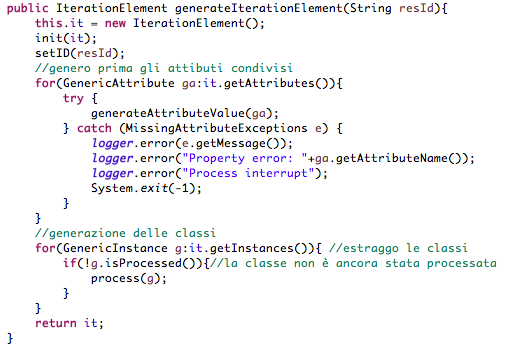
\includegraphics[width=14cm]{img/generateItEl.png}
			\caption{Funzione \emph{GenerateIterationElement()s}}\label{itelgenerator}
		\end{figure}
		
		Questa funzione riceve in ingresso l'identificativo della simulazione (il valore generato dalla query SPARQL  principale), a seguito di una fase di inizializzazione parte il processo principale.\\
		Per valorizzare tutti i valori si eseguono due cicli il primo si occupa della generazione degli attributi condivisi, ciclando sulla rispettiva lista. All'interno del ciclo per ogni attributo viene lanciata la funzione \texttt{generateAttributeValue()} che si occupa di generare il valore per l'attributo passato.\\
		Finito questo ciclo viene lanciato un altro ciclo sulla lista delle istanze che definiscono il simulatore, anche in questo caso attraverso la funzione \texttt{process()} si cicla per ogni istanza sui suoi attributi eseguendo nuovamente la funzione \texttt{generateAttributeValue()} per tutti gli attributi che compongono un'istanza.\\
		
		\begin{figure}[h!]
			\centering
			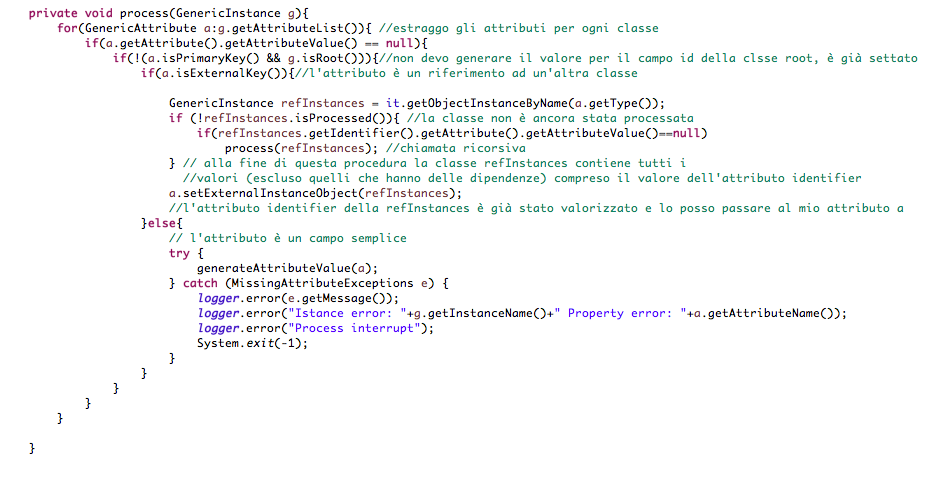
\includegraphics[width=14cm]{img/process.png}
			\caption{Funzione \emph{process()}}\label{process}
		\end{figure}
		
		Come abbiamo visto il file di configurazione può essere molto complesso, come struttura. Il valore di una proprietà può essere definito come funzione di una o più variabili oppure i parametri che definiscono una proprietà possono contenere a loro volta delle espressioni contenenti variabili.\\L'inserimento di una variabile (che in questo caso rappresenta il valore assunto da un'altra proprietà ) comporta che nel momento in cui si va a determinare il valore di quella proprietà  il valore  della proprietà alla quale la variabile fa riferimento debba essere già stato generato. Non potendo determinare a priori l'ordine di generazione delle varie proprietà questa funzione in modo sequenziale a partire dal primo elemento della lista tenta di determinare il valore, se questo ha una dipendenza funzionale da un altro valore e questo non è ancora stato calcolato allora viene richiamata in modo ricorsivo la stessa funzione sulla proprietà il cui valore non ancora stato generato. Questo procedimento viene eseguito finché tutti i valori di tutte le proprietà non sono state determinate. 
		
		\subsection{Classi per la gestione delle tipologie}
		
		Per un'efficace gestione delle diverse tipologie, al fine di ottenere un livello di astrazione elevato, è stata implementata una struttura che si rifà al paradigma del \emph{Command Pattern}. La motivazione di questa scelta è dovuta all'esigenza di avere un unica tipologia di attributo che potesse generare qualsiasi tipo di dato e dall'esigenza di poter aggiungere nuove tipologie di dato in corso d'opera senza aumentare la complessità del codice, mantenendo il sistema scalabile.
		
		Per ogni diversa tipologia di dato ci sono due aspetti da considerare: 
		\begin{enumerate}
			\item ogni tipologia ha un diverso modo di generare il valore a partire dai dati in ingresso;
			\item ogni tipologia necessita di diversi parametri in ingresso.
		\end{enumerate}
		Le classi che intervengo in questa fase sono le classi \texttt{GenericAttribute} e \texttt{GenericInstance}. Le prime due sono le classiche riprendono la struttura degli oggetti XML visti in precedenza (crf. Capitolo \ref{xml}). Queste classi contengono degli attributi accessori utili al processo iterativo, vengono generate a partire da un oggetto di tipo \texttt{Tree} e sono le classi utilizzate all'interno del processo di iterazione delle triple visto nel paragrafo precedente. Un aspetto fondamentale della classe \texttt{GenericAttribute} è che a differenza della classe \texttt{prop} (della quale riprende gran parte della struttura e scopo) non possiede tanti attributi quanti sono quelli in essa definiti (vedi figura \ref{treeClass}). La classe \texttt{prop} ha come attributi tutti gli elementi XML del file di configurazione, tutti questi attributi non sono presenti nella classe \texttt{GenericAttribute}. Questi sono stati inseriti all'interno di una \texttt{HashMap} sotto forma di nome dell'attributo e valore. Tramite questa implementazione si risolve il problema b) citato sopra, così facendo basterà passare alla funzione di generazione del valore l'intera mappa, sarà poi compito delle funzioni specifiche di ogni tipologia recuperare i valori a lei necessari per determinare il valore d'uscita. \\Così facendo si mantiene  il sistema scalabile, in quanto l'aggiunta di una nuova tipologia comporterebbe solo la sua definizione all'interno delle classi che compongono l'oggetto \texttt{Tree}, mentre la mappa è popolata in modo automatico al momento della costruzione dell'oggetto.\\
		\\
		Il valore dell'attributo è generato all'interno della classe\\ \texttt{generateAttributrValue}, questa è la funzione che ha il compito di assegnare il valore all'attributo.\\
		La funzione è eseguita su di un attributo e se questo è un espressione oppure un suo parametro lo è si eseguono dei passi per la sua valorizzazione.\\ Anche in questo caso se il valore che stiamo cercando dipende da un attributo che non è ancora stato generato, si richiama la funzione stessa su quell'attributo in modo ricorsivo. Se l'attributo non contiene espressioni e dipendenze o queste sono state risolte tutte si può richiamare  la funzione che a partire dall'attributo ne genera il valore.\\
		Nel caso in cui l'attributo fosse definito di tipo \texttt{foregoing}  o di tipo \\ \texttt{previusState}, all'interno di questa funzione sono eseguiti tutti i procedimenti per acquisire il valore recuperandolo rispettivamente da un record generato in precedenza all'interno della solita esecuzione ,per il caso \texttt{foregoing}, oppure andando a recuperare un valore generato in esecuzioni precedenti per il caso \texttt{previusState}. Una volta recuperato il valore questo viene assegnato all'attributo in oggetto, qualora non si dovesse riuscire a recuperare il valore verrebbe usato il quello di default, specificato nel file di configurazione.\\
		\newline
		Al termine di tutti questi passi tutte le dipendenze dei parametri (se esistono) sono state risolte, ed è dunque possibile procedere con la generazione del valore.
		Questo passo è eseguito dalla funzione \texttt{generateValue()} la quale vuole in ingresso la tipologia di attributo e la mappa degli attributi. Attraverso la tipologia si risale alla funzione specifica e questa utilizzando solo i parametri a lei necessari genera il valore per quell'attributo.
		\texttt{GenericTypeMap} e \texttt{GenericCommand} sono le due classi che implementano questo meccanismo, un oggetto \texttt{GenericTypeMap} è definito come attributo statico della classe \texttt{GenericAttribute} e implementa un \emph{Singleton Pattern} e all'interno di esso è definito un oggetto della classe \texttt{GenericCommand} che implementa il \emph{Command Pattern}.
		
			
			\begin{figure}[h!]
				\centering
				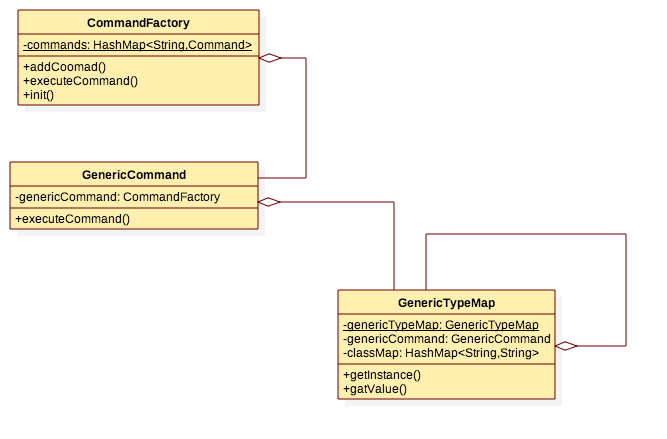
\includegraphics[width=14cm]{img/genericCommand.png}
				\caption{Class Diagram della classe GenericTypeMap}\label{genericTypeMap}
			\end{figure}
		
		\newpage
		\begin{figure}[h!]
			\centering
			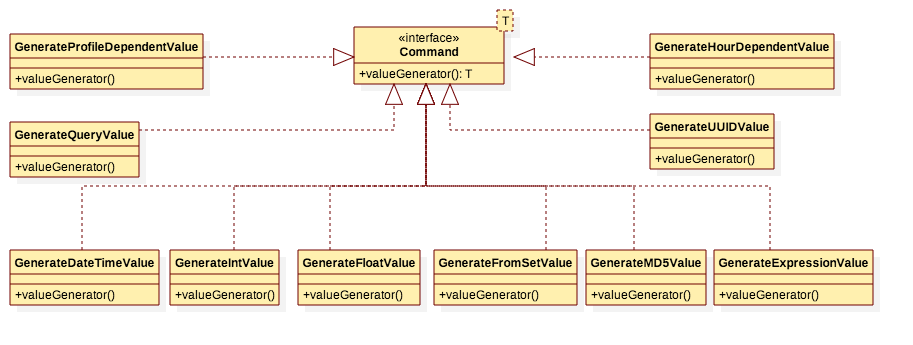
\includegraphics[width=14cm]{img/command.png}
			\caption{Varie implementazioni dell'interfaccia Command}\label{command}
		\end{figure}
		
		
		\begin{figure}[h!]
			\centering
			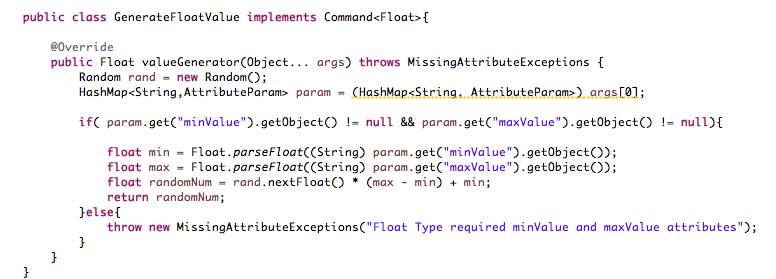
\includegraphics[width=14cm]{img/generatefloatvalue.png}
			\caption{Esempio di una implementazione dell'interfaccia}\label{floatValue}
		\end{figure}
		
		Ognuna delle classi che implementano l'interfaccia definisce un diverso modo di generare un valore ed ognuna di esse è inserita nella mappa \emph{commands} dell'oggetto \texttt{CommandFactory}.
		\newpage
			\begin{figure}[h!]
				\centering
				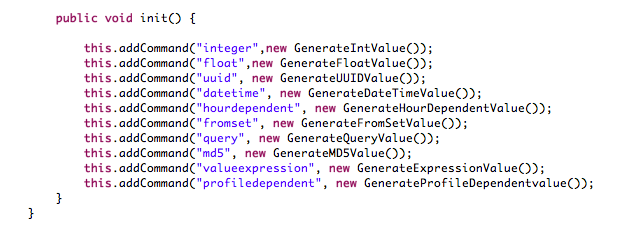
\includegraphics[height=4.3cm]{img/init.png}
				\caption{inizializzazione della mappa}\label{init}
			\end{figure}
		
		
		Tramite l'utilizzo di questa mappa a partire dal valore della tipologia che viene passata alla funzione \texttt{generateValue()} si ricava l'oggetto di tipo command che implementa il metodo \emph{valueGenerator()} per quella particolare tipologia.
\newpage
\appendix
\section{Appendice}
\subsection{Esempio di File di Configurazione}
Riprendendo l'esempio dei sensori di parcheggio citato nel paragrafo precedente, in questa sezione sarà mostrato un esempio del file di configurazione necessario per generare la simulazione relativa ad una campionatura di tale sensore (cfr. figura \ref{carparksensor}).

\begin{figure}[h!]
	\centering
	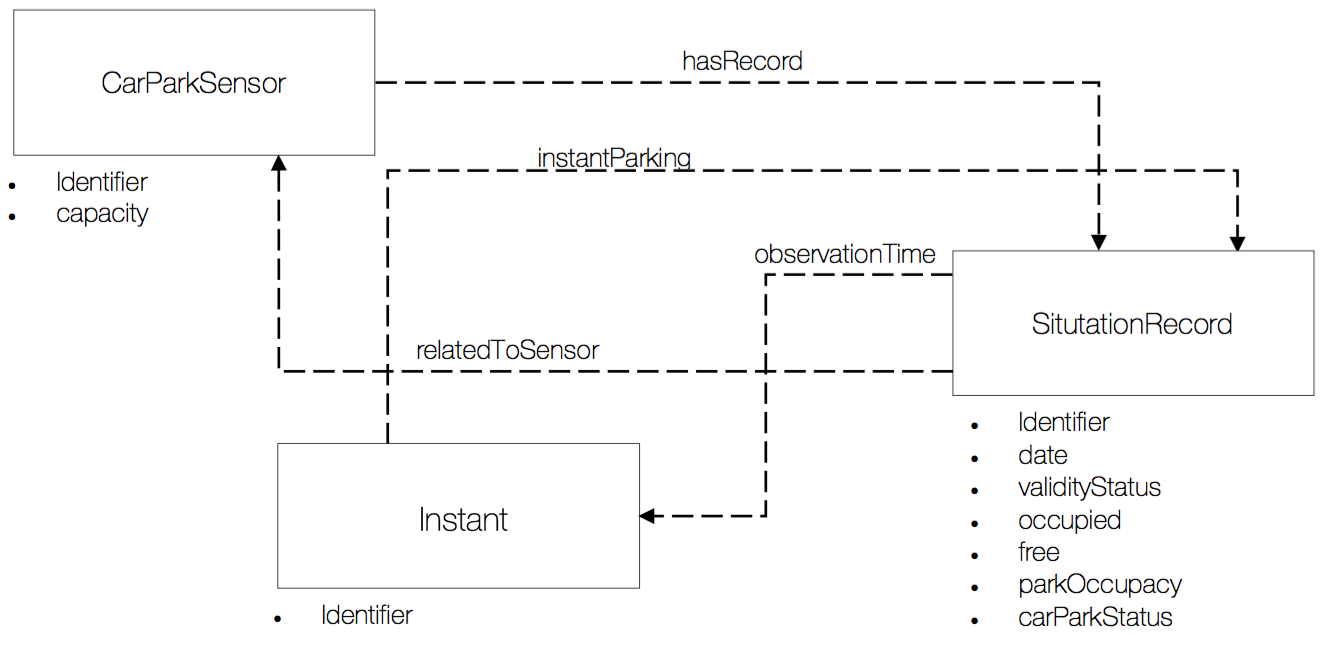
\includegraphics[width=14cm]{img/CPSschema.png}
	\caption{Schema delle classi RDF  dei sensori di parcheggio}\label{carparksensorschema}
\end{figure}
A partire dallo schema in figura il file \emph{.xml} per la generazione delle triple è il seguente:\\

\begin{figure}[h!]
	\centering
	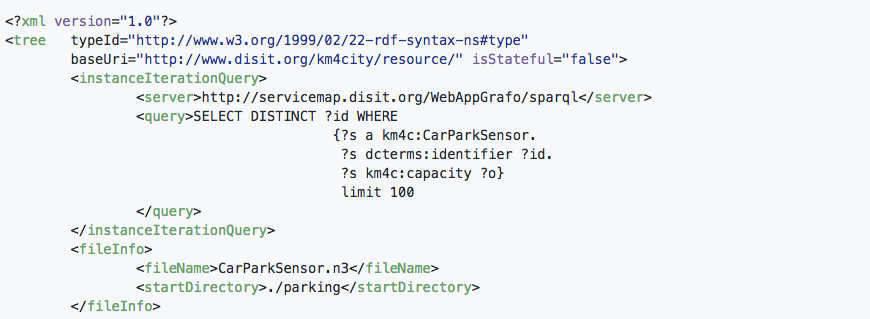
\includegraphics[width=14cm]{img/esempio_p1.png}
	\caption{Definizione della query di iterazione e de file di output}\label{esempio1}
\end{figure}
Nel \texttt{tree} si dichiarano rispettivamente la \texttt{uri} che conterrà il tipo dell'istanza e con \texttt{baseUri}, la stringa che definisce la prima parte del soggetto alla quale verrà aggiunto poi l'identificativo della risorsa. Per ogni istanza si può definire una \texttt{baseUri} diversa specificando tale attributo nella definizione dell'istanza (in caso contrario viene utilizzata quella specificata nel \texttt{tree}).
La proprietà \texttt{isStateful=''false''} specifica che queste simulazioni sono senza memoria.\\
\newline
All'interno dell'elemento \texttt{instanceIterationQuery} troviamo la definizione della query sulla quale si dovrà iterare. La query qui definita dovrà restituire sull'attributo \texttt{id} una lista di elementi che saranno l'identificativo delle risorse sulle quali verranno generate le simulazioni.\\
Nell'elemento \texttt{fileInfo} andiamo a definire la directory di partenza all'interno della quale creare le cartelle contenenti il file \emph{.n3} e il nome del file di uscita.\\
Finita la fase iniziale dove sono definite le informazioni generali si passa a specificare la struttura di ogni istanza, seguendo lo schema di figura \ref{carparksensor}. Per questa simulazione si devono definire tre istanze (\emph{CarParkSensor}, \emph{Instant} e \emph{SituationRecord}).\\
Le definizioni delle istanze sono inserite all'interno dell'elemento\\ \texttt{iterationElement}.\\
\begin{figure}[h!]
	\centering
	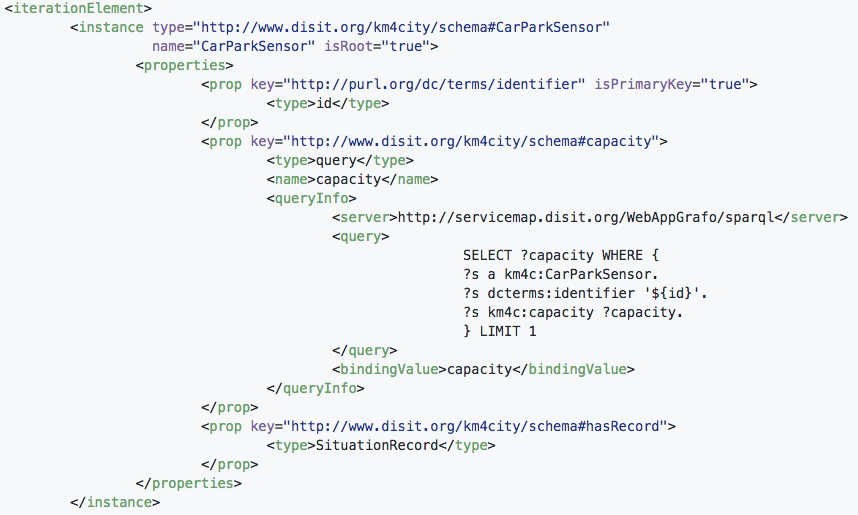
\includegraphics[width=14cm]{img/esempio_p2.png}
	\caption{Definizioni dell'istanza CarParkSensor}\label{esempio2}
\end{figure}
\\All'interno dell'elemento \texttt{instance} troviamo la definizione: dell'oggetto, il cui predicato identifica il tipo dell'istanza, del nome, dell'istanza e se questa istanza è \emph{root}.
A seguito troviamo la definizione di tutte le proprietà della classe (all'interno dell'elemento \texttt{properties}).
La prima proprietà definisce l'identificativo dell'istanza che essendo \emph{root} conterrà l'elemento estratto dalla query.\\
La seconda proprietà definisce l'attributo \emph{capacity} che rappresenta la capacità totale del parcheggio. Questo valore è ricavato tramite una query dove viene estratto il valore di capacità del sensore in oggetto. All'interno della query è stato inserito il carattere speciale \$\{id\}\footnote{La variabile \$\{id\}  insieme alla variabile \$\{index\} sono variabili di sistema e contengono rispettivamente l'id dell'iterazione corrente e l'indice dell'iterazione corrente} che contiene l'identificativo della risorsa nell'iterazione in corso.\\
Infine definiamo la proprietà \emph{hasRecord} che è un riferimento ad una istanza. Questa definizione viene fatta specificando nell'attributo \texttt{type} il nome dell'istanza a cui fare rifermento. Il valore restituito sarà il valore dell'identificativo di questa.
\newpage
\begin{figure}[h!]
	\centering
	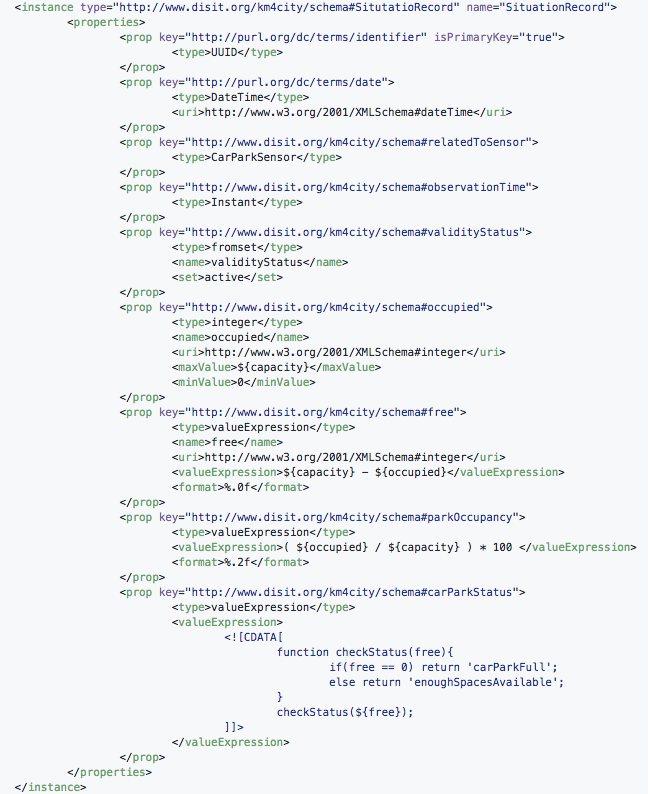
\includegraphics[width=14cm]{img/esempio_p3.png}
	\caption{Definizioni dell'istanza SituationRecord}\label{esempio3}
\end{figure}

In figura \ref{esempio3} è mostrata la definizione per l'istanza \emph{SituationRecord} con tutte le rispettive proprietà. In modo analogo al caso precedente anche in questo caso sono state definite la proprietà \texttt{identifier} e le proprietà che si riferiscono ad altre istanze (\texttt{Instant} e \texttt{CarParkSensor}) ed a seguito tutte le altre classi che definiscono questa istanza.\\
All'interno di questa istanza si fa un uso molto frequente di variabili ed espressioni (dovuto alla natura delle proprietà del sensore). Le variabili possono essere usate sia all'interno di espressioni regolari sia come parametri per la determinazione dei valori come nel caso della proprietà \texttt{occupied}, il cui valore deve essere un numero casuale tra 0 e il numero totale di posti di quel parcheggio (per ottenere questo valore si utilizza la variabile \$\{capacity\} che fa riferimento all'omonima proprietà definita nell'istanza precedente). \\
Per quanto riguarda le espressioni, di particolare interesse è la definizione di \emph{carParkStatus} dove al suo interno è stato definito del codice Javascript.\\
\begin{figure}[h!]
	\centering
	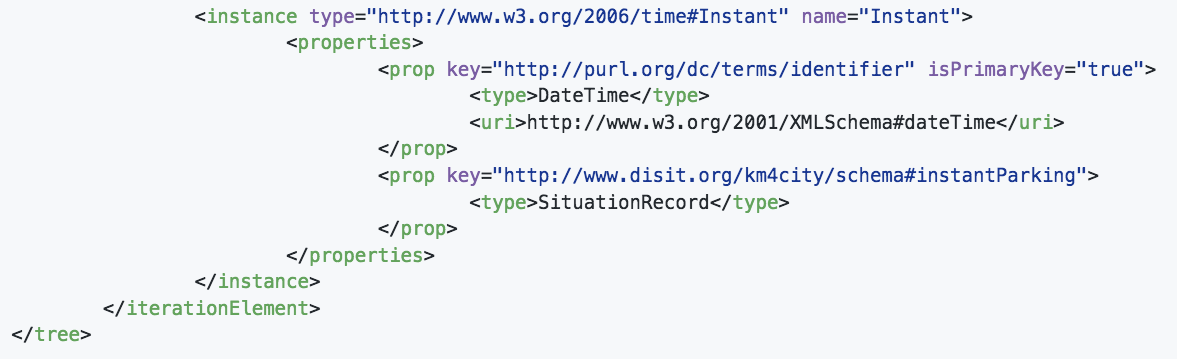
\includegraphics[width=14cm]{img/esempio_p4.png}
	\caption{Definizioni dell'istanza Instant}\label{esempio4}
\end{figure}

Infine in figura \ref{esempio4} è mostrata la definizione dell'istanza \emph{Instant} che completa la caratterizzazione di un sensore di parcheggio all'interno dell'ontologia di \emph{km4city}
\newpage
\subsection{Aggiunta di una nuova tipologia}
In questa sezione sono illustrati tutti i passaggi necessari per aggiungere una nuova tipologia al sistema.\\
L'iter per l'aggiunta di una nuova tipologia prevede i seguenti passaggi:
 \begin{enumerate}
 	\item Aggiunta degli attributi alle classi del \texttt{Tree}.
 	\item Aggiunta della nuova tipologia alla lista di tipi personalizzati.
 	\item Implementazione della logica di generazione del valore d'uscita.
 \end{enumerate}
 \subsubsection{Definizione degli attributi}
 Il primo passo da compiere è quello di fare in modo che i nuovi elementi inseriti nel file di configurazione XML siano correttamente serializzati all'interno delle apposite classi.
 Gli attributi che definiscono il nostro novo tipo devono essere dichiarati all'interno della classe \texttt{Prop} insieme ai rispettivi metodi \emph{getter} e \emph{setter}. In questo modo la nuova tipologia può essere correttamente serializzata all'interno dell'oggetto \texttt{Tree}.
 \subsubsection{Aggiunta della nuova tipologia}
 All'interno della classe \texttt{TypeMap} in una \emph{HashMap} è definita la lista di tipologie personalizzate e il relativo tipo di valore restituito.
  \begin{figure}[h!]
  	\centering
  	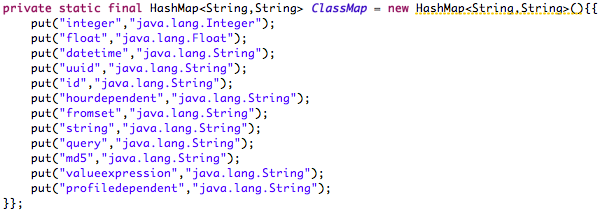
\includegraphics[height=4cm]{img/typemap.png}
  	\caption{Mappatura dei tipi personalizzati}\label{typeMap}
  \end{figure}
  \\
  Nella mappa sopracitata è necessario inserire il nuovo tipo di dato (il valore che compare all'interno del tag \emph{type}) e la tipologia di dato in uscita.\\
  \subsubsection{Implementazione della funzione di generazione del valore}
  L'ultimo passaggio richiede la definizione della funzione di generazione del valore, per farlo è necessario creare una nuova classe che implementa l'interfaccia \emph{Command} e ridefinire il metodo \texttt{valueGenerator(Object... args)}. All'interno dell'oggetto \emph{args} (che contiene un solo valore) è presente la lista dei parametri definiti per l'attributo in questione sotto forma di HashMap<chiave,valore>, tramite questo oggetto è possibile ricavare i parametri definiti nell'XML di cui abbiamo bisogno per poter generare il valore d'uscita.\\
  Infine una volta definita questa classe è necessario associarla al nuovo tipo aggiungendo un record nella mappa del \texttt{CommandFactory} (vedi figura \ref{init}).

\end{document}